\chapter{ANALISI DI SITI ESISTENTI}
\section{Everything Dinosaur}
\href{https://www.everythingdinosaur.com/}{\textbf{everythingdinosaur.com}}
\\
Un negozio online specializzato in giocattoli, modellini e articoli educativi legati ai dinosauri. Offrono una vasta selezione di prodotti e sono conosciuti per la loro attenzione ai dettagli scientifici.
\\
\textbf{Sito da browser web:}
\begin{figure}[H]
        \centering
        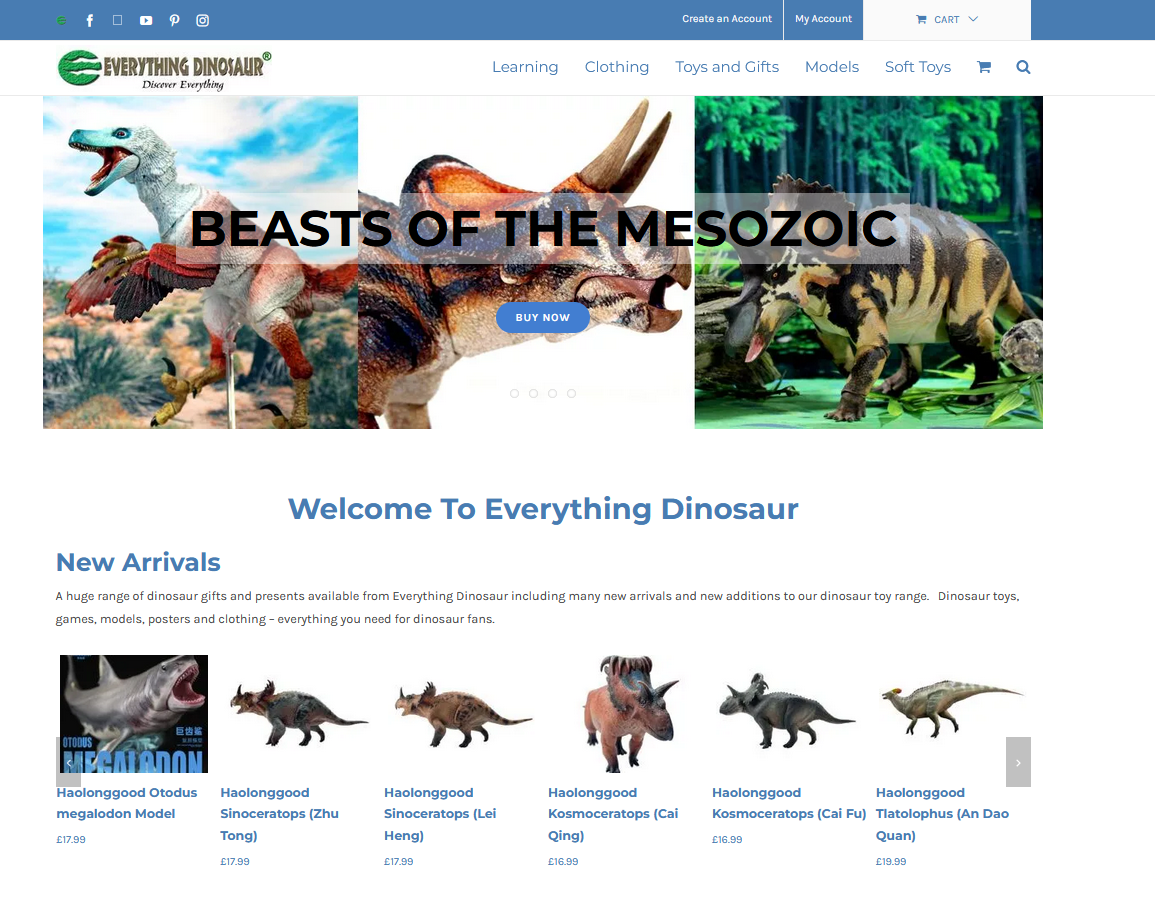
\includegraphics[width=0.60\textwidth]{immagini/everythingdinosaurpng.png}
        \caption{Everything dinosaur visualizzazione da desktop}
    \end{figure}
    
\textbf{Sito da mobile:}
\begin{figure}[H]
        \centering
        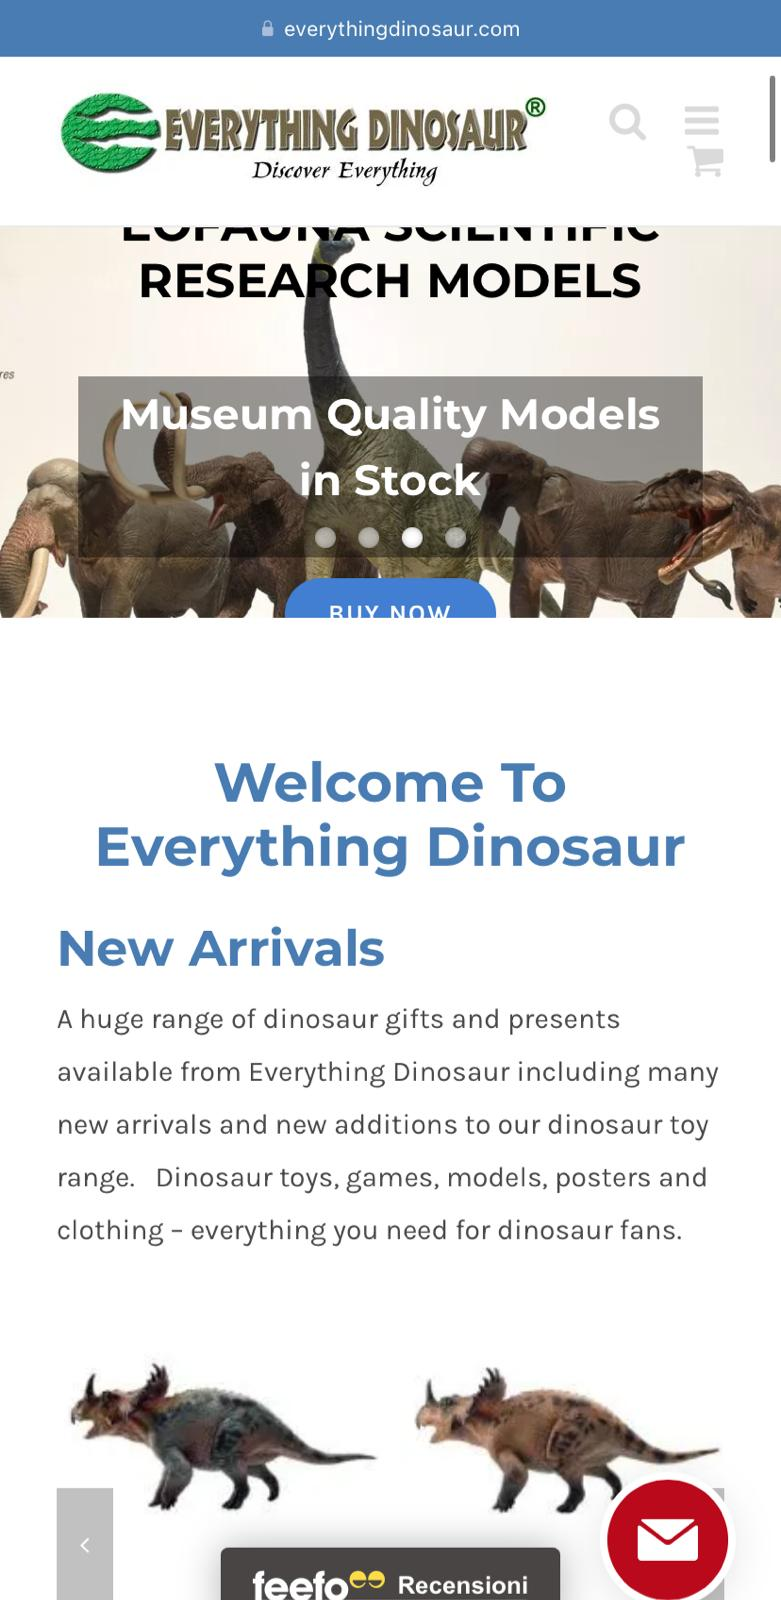
\includegraphics[width=0.45\textwidth]{immagini/everythingdinosaur_mobile.jpg}
        \caption{Everything dinosaur visualizzazione da mobile}
    \end{figure}

Il sito si presenta con un'interfaccia semplice, anche se non molto intuitiva. L'header è composto dai contatti e dal logo del sito web, mentre nella parte destra è possibile creare un account, effettuare il login e visualizzare il carrello. Gli utenti non registrati, possono esplorare il sito e visualizzare i prodotti, ma hanno accesso limitato a funzionalità avanzate come il salvataggio degli articoli nel carrello per un accesso futuro. Tuttavia possono effettuare un ordine e procedere al check-out senza dover necessariamente creare un profilo.
\\
Nel corpo del sito troviamo un carosello composto da tre immagini con scorrimento manuale. Nella parte inferiore destra troviamo varie categorie, come articoli da regalo, vestiti, modellini, e una lente d'ingrandimento per cercare prodotti all'interno del sito. Scorrendo ulteriormente, troviamo un carosello di prodotti con i nuovi arrivi e i vari modellini suddivisi in base alle caratteristiche distintive di ogni dinosauro. Ogni prodotto ha una pagina dedicata con una descrizione dettagliata, immagini di alta qualità e informazioni aggiuntive come dimensioni, materiali e altre caratteristiche pertinenti. 
\\
Nel footer notiamo invece varie informazioni relative alla storia del sito stesso e i motivi per cui acquistare sul loro ecommerce. Più in basso troviamo la possibilità di iscriversi alla newsletter. 

\begin{figure}[H]
        \centering
        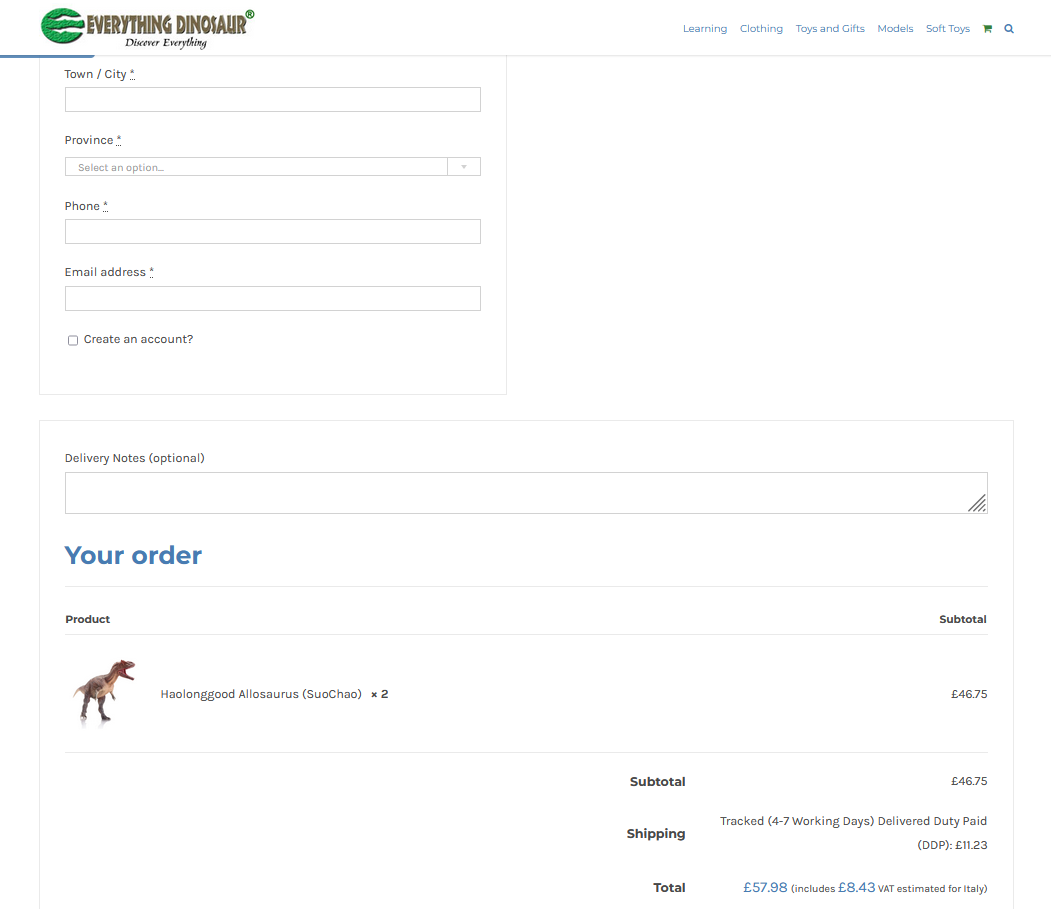
\includegraphics[width=0.80\textwidth]{immagini/everything_dinosaur_checkout.png}
        \caption{Check-out everything dinosaur}
    \end{figure}
\section{Dinosaur Corporation}
\href{https://www.dinosaurcorporation.com/}{\textbf{dinosaurcorporation.com}}
\\Dinosaur Corporation è un sito specializzato nella vendita di prodotti correlati ai dinosauri che offre una vasta selezione di giocattoli, peluche, modellini e articoli da collezione legati a questi animali. Le informazioni sono dettagliate, il servizio clienti è affidabile e le opzioni di pagamento sono sicure per soddisfare le esigenze dei suoi clienti. 
\\
\textbf{Sito da browser web:}
\begin{figure}[H]
        \centering
        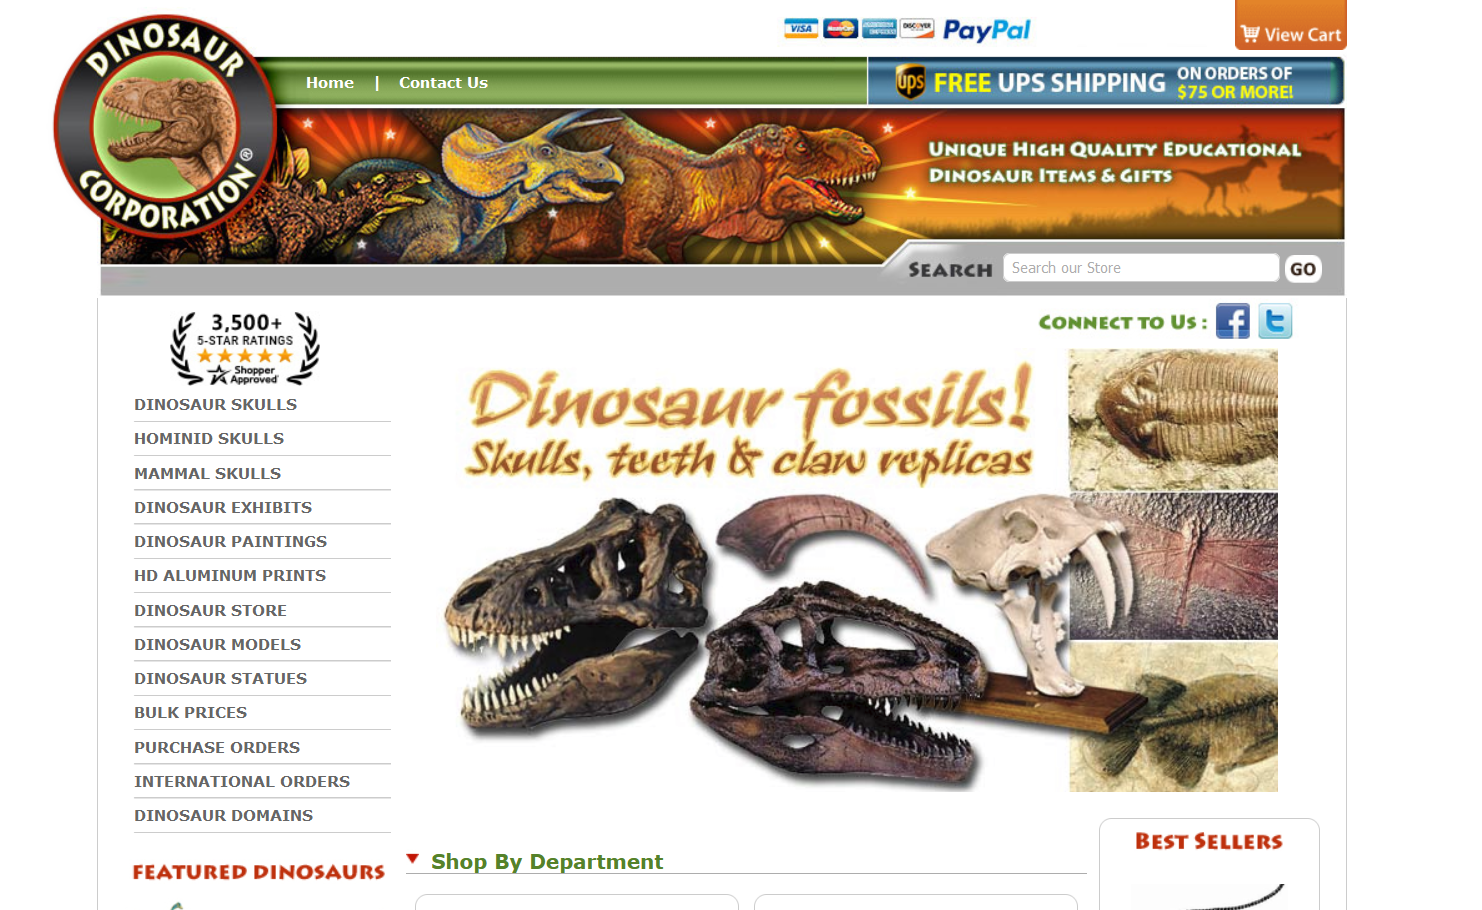
\includegraphics[width=0.60\textwidth]{immagini/dinosaurcorporation.png}
        \caption{Dinosaur corporation visualizzazione web}
    \end{figure}

\textbf{Sito da mobile:}
\begin{figure}[H]
        \centering
        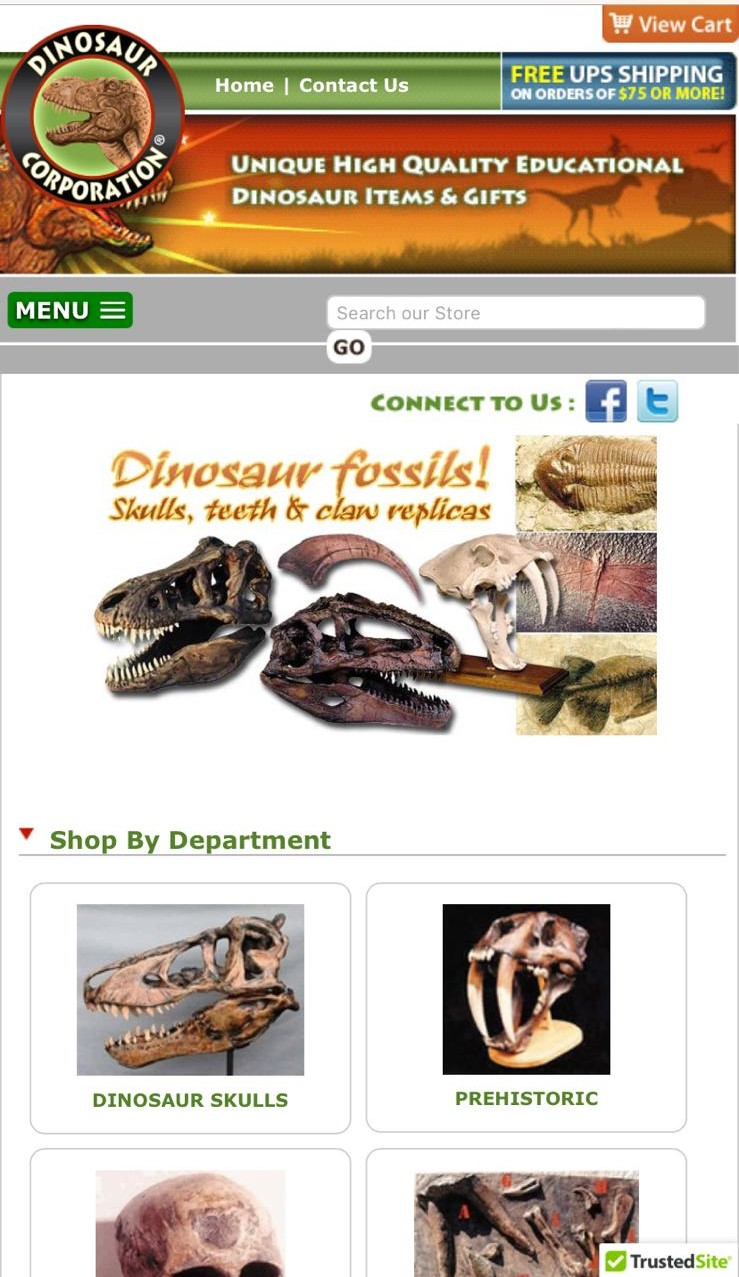
\includegraphics[width=0.45\textwidth]{immagini/dinosaurcorporation_mobile.jpg}
        \caption{Dinosaur Corporation visualizzazione da mobile}
    \end{figure}
L’homepage del sito si presenta con un’interfaccia meno moderna e per questa ragione alcuni utenti potrebbero avere difficoltà ad accedere ai prodotti offerti. Nell’header superiore è presente il logo del sito, i contatti e a destra abbiamo la possibilità di vedere il carrello. Più in basso troviamo una barra di ricerca con la quale possiamo navigare tra i vari prodotti del sito. Nella homepage troviamo i prodotti suddivisi in diverse categorie, ognuna delle quali ha un'immagine rappresentativa. Selezionando una categoria troviamo tutti i prodotti relativi a quest'ultima e la possibilità di aggiungerli direttamente al carrello. In questo sito web non è possibile effettuare una registrazione o un log-in. La schermata del carrello è la seguente, dove possiamo visualizzare la lista dei prodotti e i relativi prezzi, eventualmente possiamo vedere anche il prezzo della spedizione. 
\begin{figure}[H]
        \centering
        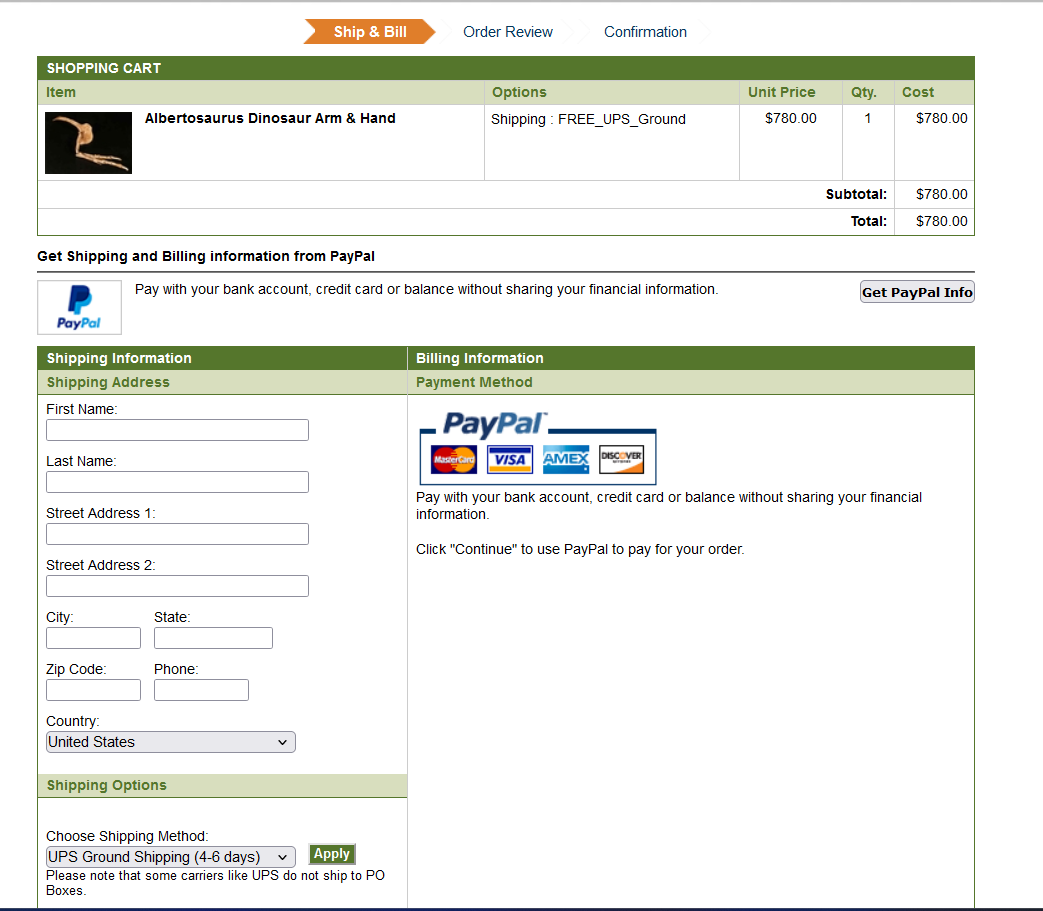
\includegraphics[width=0.70\textwidth]{immagini/dinosaur_corporation_checkout.png}
        \caption{Check-out di Dinosaur Corporation }
    \end{figure}
    
\section{Rocco Giocattoli}
\href{https://shop.roccogiocattoli.eu/brand/jurassic-world}{\textbf{roccogiocattoli.eu/brand/jurassic-world}}
\\
Rocco Giocattoli è un negozio online specializzato in modellini di Jurassic World. Il sito si presenta con un'interfaccia semplice visualizzando un header che mostra in alto a sinistra il logo, al centro una barra di ricerca per navigare all'interno del sito e a destra il carrello e l'area utente.
\\
L'homepage parte con la presentazione dei vari prodotti in catalogo e la possibilità di aggiungerli al carrello o alla lista desideri, il menù è suddiviso in varie categorie di prodotti. Inoltre è possibile filtrare tramite la barra laterale il prezzo e l'età consigliata dei vari giocattoli. 
\\
Nel footer, invece, troviamo informazioni sulle spedizioni, i pagamenti, i contatti, la storia dell'azienda e un altro collegamento all'area utente.
\\

\textbf{Sito da browser web:}
\begin{figure}[H]
        \centering
        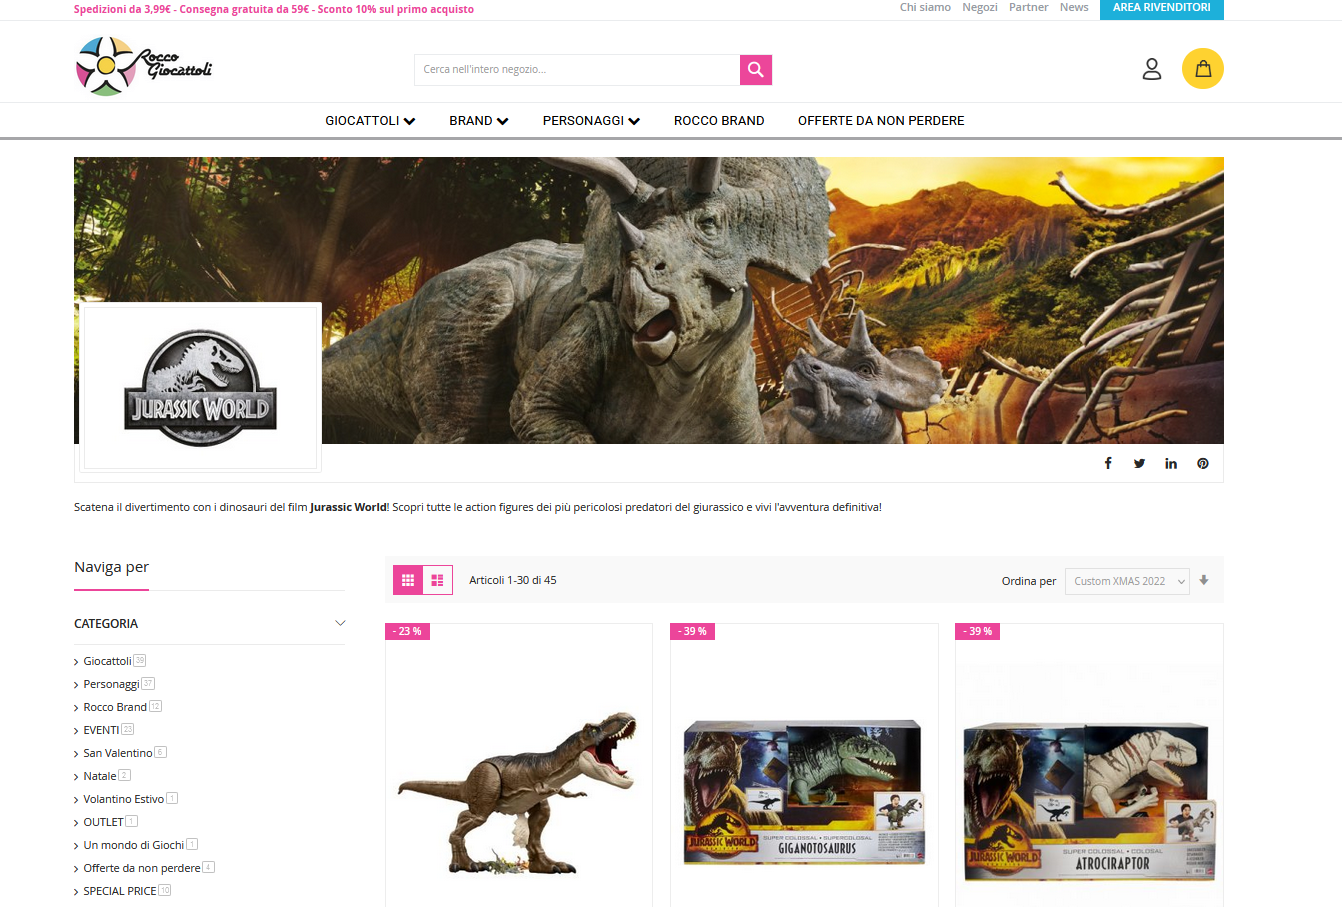
\includegraphics[width=0.50\textwidth]{immagini/roccogiocattoli.png}
        \caption{Rocco Giocattoli visualizzazione da browser web}
    \end{figure}
    
\textbf{Sito da mobile:}
\begin{figure}[H]
        \centering
        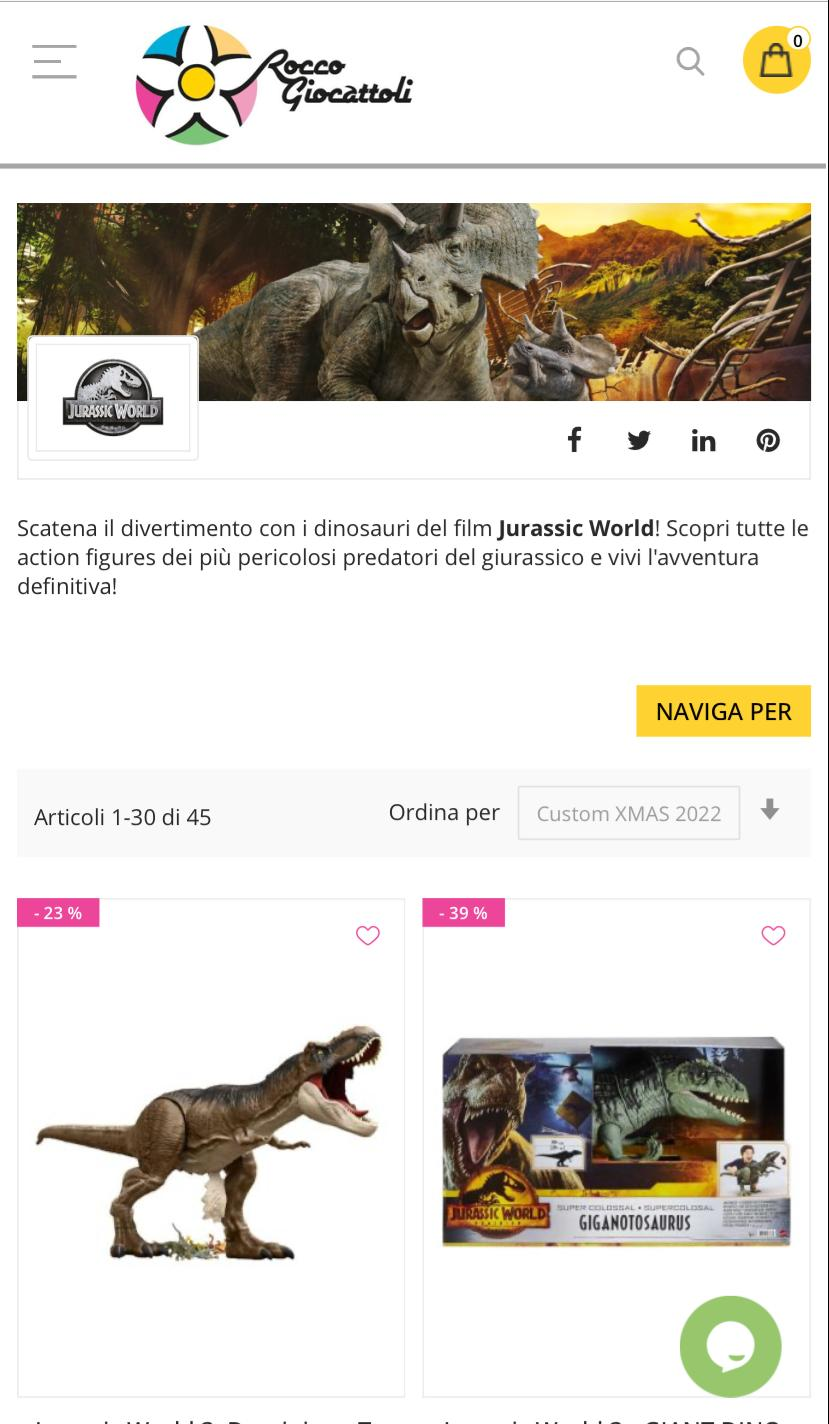
\includegraphics[width=0.35\textwidth]{immagini/roccogiocattoli_mobile.jpg}
        \caption{Rocco Giocattoli visualizzazione del sito da mobile}
    \end{figure}
Selezionando un prodotto da acquistare abbiamo la possibilità di scegliere se aggiungerlo al carrello, comprarlo subito o aggiungerlo ad un'eventuale lista dei desideri, e varie informazioni tra cui tempi di consegna e caratteristiche dell'articolo. è anche possibile lasciare una recensione, non bisogna essere registrati ne tanto meno aver fatto l'acquisto del prodotto specifico. 
\begin{figure}[H]
        \centering
        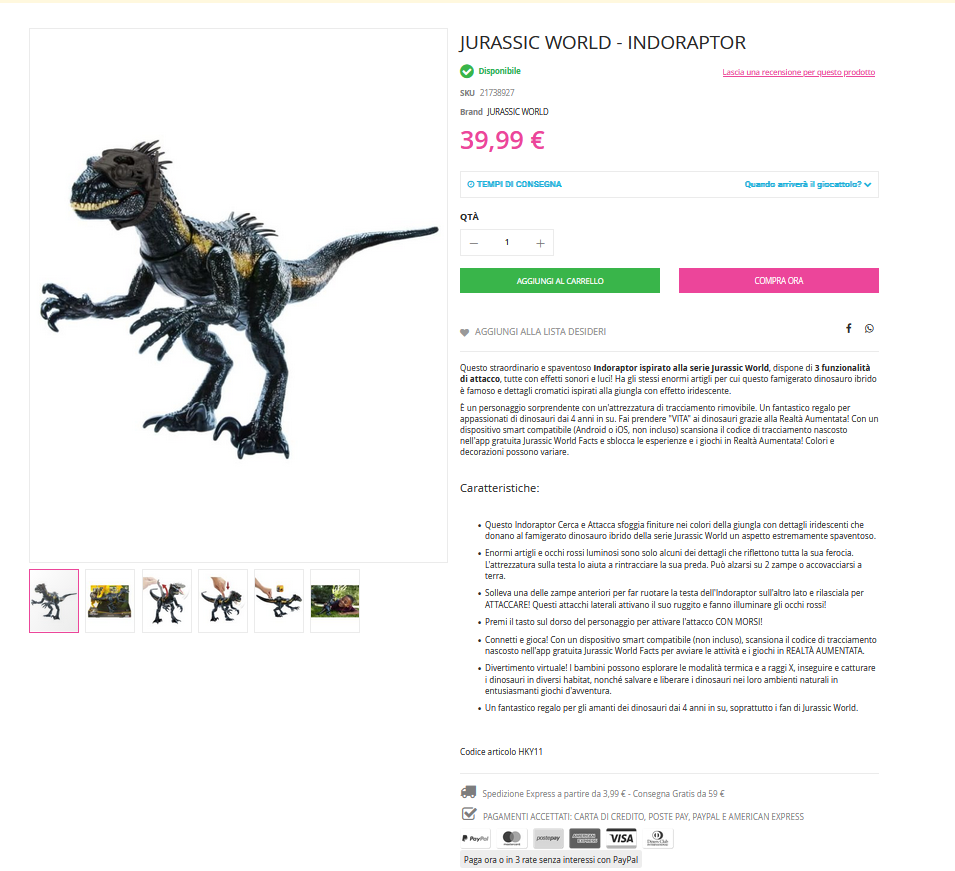
\includegraphics[width=0.5\textwidth]{immagini/prodotto_roccogiocattoli.png}
        \caption{Pagina del prodotto }
    \end{figure}
Il cliente può aggiungere prodotti al carrello senza necessariamente essere registrato o aver fatto il login, procedendo al check-out compare la seguente schermata:
 \begin{figure}[H]
        \centering
        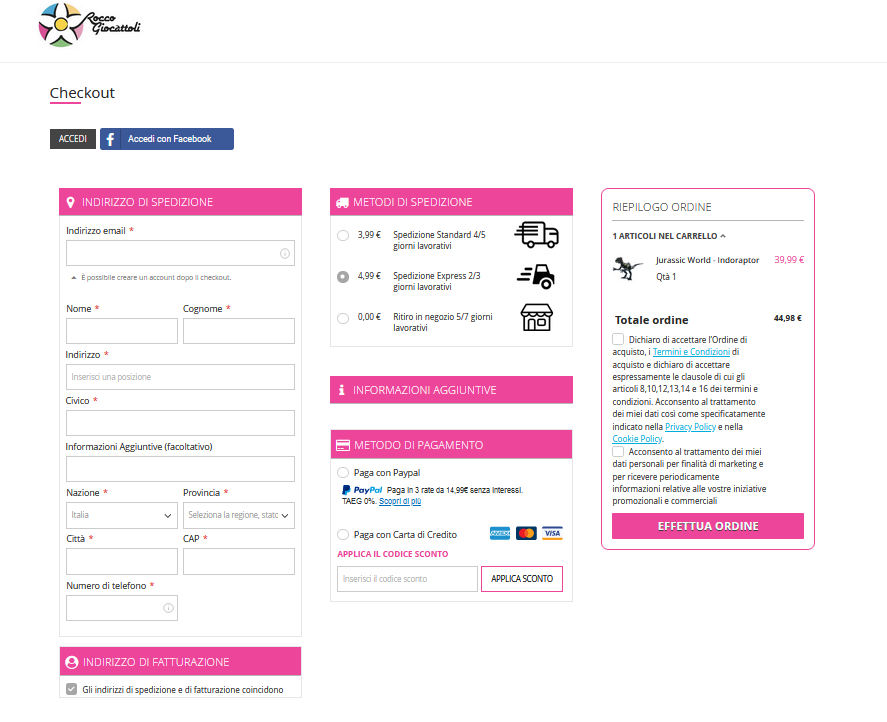
\includegraphics[width=0.55\textwidth]{immagini/check-out_roccogiocattoli.png}
        \caption{Check-out Rocco Giocattoli}
    \end{figure}
Nella sezione carrello anche se non si è registrati è possibile visualizzare la lista dei prodotti inseriti e il totale che comprende anche la spedizione.

\begin{comment}
    Il sito proposto `e un e-commerce specializzato nella vendita di dinosauri domestici,
mirato a un pubblico di appassionati di animali insoliti e originali. La piattaforma
si propone di soddisfare i bisogni dei clienti interessati all’acquisto di dinosauri
domestici come animali da compagnia o come oggetti di collezione. Offrir`a una
vasta gamma di prodotti relativi ai dinosauri, fornendo informazioni dettagliate sui
prodotti e facilitando il processo di acquisto attraverso un’interfaccia user-friendly
e sicura.
\end{comment}